\chapter{\LaTeX 使用入门}

~\LaTeX~的命令形式均为一个反斜杠后跟字母及括号,一般请在输入一个命令之后敲一个空格,以免产生未知错误。

\section{换段、换行与空格}

在~\LaTeX~中,单个的回车与空格会被忽略。

\begin{description}
 \item[换段]此处的换段指的是开启一个新段落,通过空一行(两次回车)实现段落换行,也可以通过 \verb|\par| 命令来新起一段。
 \item[换行]此处的换行指的是换行不换段,通过输入两个反斜杠也即是\verb|\\|可以实现换行,换行之后不会缩进,与上一行仍属于一个段落的内容。
 \item[空格]此处的空格指的不是键盘上敲一下空格键生成的空格,而是出现在文中的空格,例如\quad 这\quad 样,通过命令\verb|\quad|即可实现。
\end{description}

\section{标题}

\begin{tabular}{l l}
\verb|\chapter{}| & 一级标题命令\quad 形如第一章 \\
\verb|\section{}| & 二级标题命令\quad 形如1.1 \\
\verb|\subsection{}| & 三级标题命令\quad 形如1.1.1 \\
\verb|\subsubsection{}| & 四级标题命令\quad 形如1.1.1.1 \\
\end{tabular}

\section{字体调节}

\begin{tabular}{l l l}
 \verb|\textbf{}| & \textbf{成都理工大学} & 文本加粗\\
 \verb|\textit{}| & \textit{成都理工} & 文本斜体\\
 \verb|\mathbf{}| & $\mathbf{CDUT}$ & 数学环境下加粗\\
 \verb|\bm{}| & $\bm{CDUT}$ & 数学环境下加粗斜体\\
 \verb|\mathrm{}| & $\mathrm{CDUT}$ & 公式中的正体\\ 
\end{tabular}

\section{公式}

\subsection{常用数学环境}

在~\LaTeX~中撰写公式,需要给公式加上一个数学环境,下列为常用的数学环境。\\

\begin{tabular}{ll}
\toprule
环境命令 & 命令含义\quad 是否编号\\
\midrule
 \verb|\(...\)| & 行内公式\quad 不编号 \\
 \verb|$...$| & 行内公式\quad 不编号 \\
 \verb|\begin{math}...\end{math}| & 行内公式\quad 不编号 \\
 \verb|\[...\]| & 行间公式\quad 不编号 \\
 \verb|\begin{equation}...\end{equation}| & 行间公式\quad 编号 \\
 \verb|\begin{displaymath}...\end{displaymath}| & 行间公式\quad 不编号 \\
 \verb|\begin{equation*}...\end{equation*}| & 行间公式\quad 不编号 \\
\bottomrule
\end{tabular}

\subsection{公式范例}

\subsubsection{行内及行间公式}

在文中引用公式可以这么写:$a^2+b^2=c^2$这是勾股定理,它还可以表示为$c=\sqrt{a^2+b^2}$,还可以让公式单独一段并且加上编号。注意,公式前请不要空行。
\begin{equation}
\sin^2{\theta}+\cos^2{\theta}=1 \label{eq:pingfanghe}
\end{equation}

这样就可以通过添加标签在正文中引用公式,如式\eqref{eq:pingfanghe}。

\subsubsection{矩阵及多行对齐公式}

在大的数学环境内嵌套一些特定环境可以实现更加丰富的效果,下面的示例都是在\verb|\begin{equation}...\end{equation}|中嵌套。

嵌套\verb|\begin{matrix}...\end{matrix}|可实现矩阵的显示:
\begin{equation}
  \mathbf{A}=
  \left[\begin{matrix}
    1&2&3&4\\
    11&22&33&44\\
  \end{matrix}\right] \times
  \left[\begin{matrix}
    22&24\\
    32&34\\
    42&44\\
    52&54\\
  \end{matrix}\right]
\end{equation}

嵌套\verb|\begin{aligned}...\end{aligned}|可实现多行对齐的公式:
\begin{equation}
  \begin{aligned}
    f_1(x)&=(x+y)^2\\
          &=x^2+2xy+y^2
  \end{aligned}
\end{equation}

上面的形式同样也能通过嵌套\verb|\begin{split}...\end{split}|实现:
\begin{equation}
\begin{split}
A & = \frac{\pi r^2}{2} \\
 & = \frac{1}{2} \pi r^2
\end{split}
\end{equation}

在公式的对齐中,使用的都是\verb|&|字符来标定对齐位置,~\LaTeX~会将\verb|&|后的第一个字符内容对齐,在两行之间使用\verb|//|来分割。

\subsubsection{对齐方程组}

方程的对齐可以用\verb|\begin{align*}...\end{align*}|实现,这一环境作用为生成一不带编号(带*号表示不编号,去掉*号则对每行公式都编号,此规则适用大多数的数学环境)的多行对齐的方程。
\begin{align*} 
2x - 5y &=  8 \\ 
3x + 9y &=  -12
\end{align*}

下面是一个灵活插入\verb|&|以实现更复杂的方程组排列对齐的例子:
\begin{align*}
x&=y           &  w &=z              &  a&=b+c\\
2x&=-y         &  3w&=\frac{1}{2}z   &  a&=b\\
-4 + 5x&=2+y   &  w+2&=-1+w          &  ab&=cb
\end{align*}

\subsubsection{长公式}

当一个公式过长时可以通过\verb|\begin{multline*}...\end{multline*}|将其分割为两行显示,带*号表示此环境不对公式进行编号。

\begin{multline*}
p(x) = 3x^6 + 14x^5y + 590x^4y^2 + 19x^3y^3- 12x^5y^7 - 12y^3 + 2y^4 - a^2b^5\\ 
- 12x^2y^4 - 12xy^5 + 2y^6 - a^3b^3
\end{multline*}

\section{图片}

\subsection{\LaTeX 中的图}

\LaTeX 环境下可以使用常见的图片格式:JPEG、PNG、PDF、EPS等。当然也可以使用\LaTeX 直接绘制矢量图形,可以参考pgf/tikz等包中的相关内容。需要注意的是,无论采用什么方式绘制图形,首先考虑的是图片的清晰程度以及图片的可理解性,过于不清晰的图片将可能会浪费很多时间。

\subsection{使用TikZ绘图}

在~\LaTeX~使用TikZ绘图可以呈现绝大多数能够精确描述的矢量图,此处仅做示范,具体学习如何使用TikZ宏包绘制图形,参见\unlink{https://www.latexstudio.net/archives/1398.html}{绘图学习笔记}以及\unlink{https://njuwfang.github.io/2018/10/23/Latex-Tikz/}{用PGF/TikZ画图}。

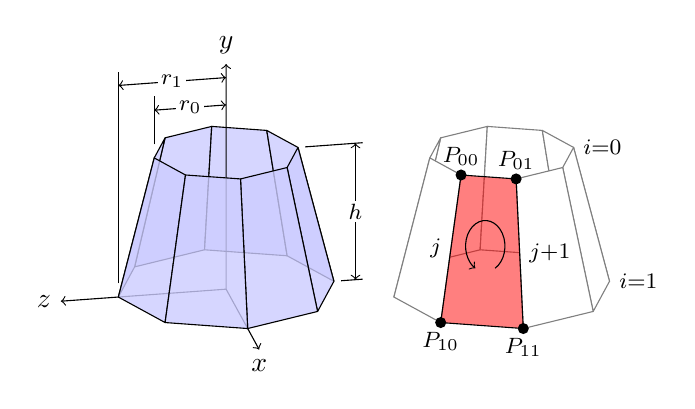
\begin{tikzpicture}[join=round]
    \tikzstyle{conefill} = [fill=blue!20,fill opacity=0.8]
    \tikzstyle{ann} = [fill=white,font=\footnotesize,inner sep=1pt]
    \tikzstyle{ghostfill} = [fill=white]
         \tikzstyle{ghostdraw} = [draw=black!50]
    \filldraw[conefill](-.775,1.922)--(-1.162,.283)--(-.274,.5)
                        --(-.183,2.067)--cycle;
    \filldraw[conefill](-.183,2.067)--(-.274,.5)--(.775,.424)
                        --(.516,2.016)--cycle;
    \filldraw[conefill](.516,2.016)--(.775,.424)--(1.369,.1)
                        --(.913,1.8)--cycle;
    \filldraw[conefill](-.913,1.667)--(-1.369,-.1)--(-1.162,.283)
                        --(-.775,1.922)--cycle;
    \draw(1.461,.107)--(1.734,.127);
    \draw[arrows=<->](1.643,1.853)--(1.643,.12);
    \filldraw[conefill](.913,1.8)--(1.369,.1)--(1.162,-.283)
                        --(.775,1.545)--cycle;
    \draw[arrows=->,line width=.4pt](.274,-.5)--(0,0)--(0,2.86);
    \draw[arrows=-,line width=.4pt](0,0)--(-1.369,-.1);
    \draw[arrows=->,line width=.4pt](-1.369,-.1)--(-2.1,-.153);
    \filldraw[conefill](-.516,1.45)--(-.775,-.424)--(-1.369,-.1)
                        --(-.913,1.667)--cycle;
    \draw(-1.369,.073)--(-1.369,2.76);
    \draw(1.004,1.807)--(1.734,1.86);
    \filldraw[conefill](.775,1.545)--(1.162,-.283)--(.274,-.5)
                        --(.183,1.4)--cycle;
    \draw[arrows=<->](0,2.34)--(-.913,2.273);
    \draw(-.913,1.84)--(-.913,2.447);
    \draw[arrows=<->](0,2.687)--(-1.369,2.587);
    \filldraw[conefill](.183,1.4)--(.274,-.5)--(-.775,-.424)
                        --(-.516,1.45)--cycle;
    \draw[arrows=<-,line width=.4pt](.42,-.767)--(.274,-.5);
    \node[ann] at (-.456,2.307) {$r_0$};
    \node[ann] at (-.685,2.637) {$r_1$};
    \node[ann] at (1.643,.987) {$h$};
    \path (.42,-.767) node[below] {$x$}
        (0,2.86) node[above] {$y$}
        (-2.1,-.153) node[left] {$z$};
    % Second version of the cone
    \begin{scope}[xshift=3.5cm]
    \filldraw[ghostdraw,ghostfill](-.775,1.922)--(-1.162,.283)--(-.274,.5)
                                   --(-.183,2.067)--cycle;
    \filldraw[ghostdraw,ghostfill](-.183,2.067)--(-.274,.5)--(.775,.424) 
                                   --(.516,2.016)--cycle;
    \filldraw[ghostdraw,ghostfill](.516,2.016)--(.775,.424)--(1.369,.1)
                                   --(.913,1.8)--cycle;
    \filldraw[ghostdraw,ghostfill](-.913,1.667)--(-1.369,-.1)--(-1.162,.283)
                                   --(-.775,1.922)--cycle;
    \filldraw[ghostdraw,ghostfill](.913,1.8)--(1.369,.1)--(1.162,-.283)
                                   --(.775,1.545)--cycle;
    \filldraw[ghostdraw,ghostfill](-.516,1.45)--(-.775,-.424)--(-1.369,-.1)
                                   --(-.913,1.667)--cycle;
    \filldraw[ghostdraw,ghostfill](.775,1.545)--(1.162,-.283)--(.274,-.5)
                                   --(.183,1.4)--cycle;
    \filldraw[fill=red,fill opacity=0.5](-.516,1.45)--(-.775,-.424)--(.274,-.5)
                                         --(.183,1.4)--cycle;
    \fill(-.775,-.424) circle (2pt);
    \fill(.274,-.5) circle (2pt);
    \fill(-.516,1.45) circle (2pt);
    \fill(.183,1.4) circle (2pt);
    \path[font=\footnotesize]
            (.913,1.8) node[right] {$i\hbox{$=$}0$}
            (1.369,.1) node[right] {$i\hbox{$=$}1$};
    \path[font=\footnotesize]
            (-.645,.513) node[left] {$j$}
            (.228,.45) node[right] {$j\hbox{$+$}1$};
    \draw (-.209,.482)+(-60:.25) [yscale=1.3,->] arc(-60:240:.25);
    \fill[black,font=\footnotesize]
                    (-.516,1.45) node [above] {$P_{00}$}
                    (-.775,-.424) node [below] {$P_{10}$}
                    (.183,1.4) node [above] {$P_{01}$}
                    (.274,-.5) node [below] {$P_{11}$};
    \end{scope}
\end{tikzpicture}

\subsection{插入图片}

插入图片的命令为\verb|\includegraphics[]{}|,方括号[]里是控制图片大小以及角度的控制命令,大括号{}里是所插入图片的文件名(注意,一定要把图片放到figures文件夹里去)。
\subsection{插图控制}

这里罗列一些插入图片时常用的控制命令:

\begin{tabular}{ll}
\verb|scale=...| & 等比例缩放 \\
\verb|width=..., height=...| & 宽和高 \\
\verb|width=...\textwidth| & 与文本宽度成比例\\
\verb|angle=...| & 旋转(顺时针为负数,逆时针为正数,单位度)\\
\end{tabular}

\subsection{图片环境}

在\LaTeX 中插入的图片需要放入一个名为浮动体的环境中以便于\LaTeX 进行排版,其一般形式如下:

\verb|\begin{figure}[!htbp]|\par
\verb|\centering|\par
\verb|\includegraphics[]{}|\par
\verb|\chartname{图名}|\par
\verb|\label{图片标签}|\par
\verb|\end{figure}|

简单来说,\verb|\begin{figure}...\end{figure}|是一对,就像c语言里的if和end一样,
在\verb|\begin{figure}...\end{figure}|之间为图片浮动体。

\verb|\chartname{图名}|这一命令即是对插入的图片取一个图名,此为笔者模板中自定义的新命令用于行使传统的\verb|\caption{}|命令的职能。

\verb|\label{图片标签}|这个命令紧跟在图名命令后,作用是给图片加一个标签,所谓标签也即是引用的时候你输入这个标签就能够引用图名了。

\verb|[htbp]|选项意即是浮动体位于此处、页顶、页底、独立一页。位置选项中加上 ! 号将使浮动体相对更靠近文字或靠前出现。

\subsection{插图范例}

在论文写作过程中常需要插入图片,一般来说,科学论文的图片,不要出现并列排在一起并且编号的,一般一个图独立占一行,一个图可以包含多个子图。

下面做一些简单的示例(代码见左侧工作区):

\begin{figure}[htb]
    \centering
     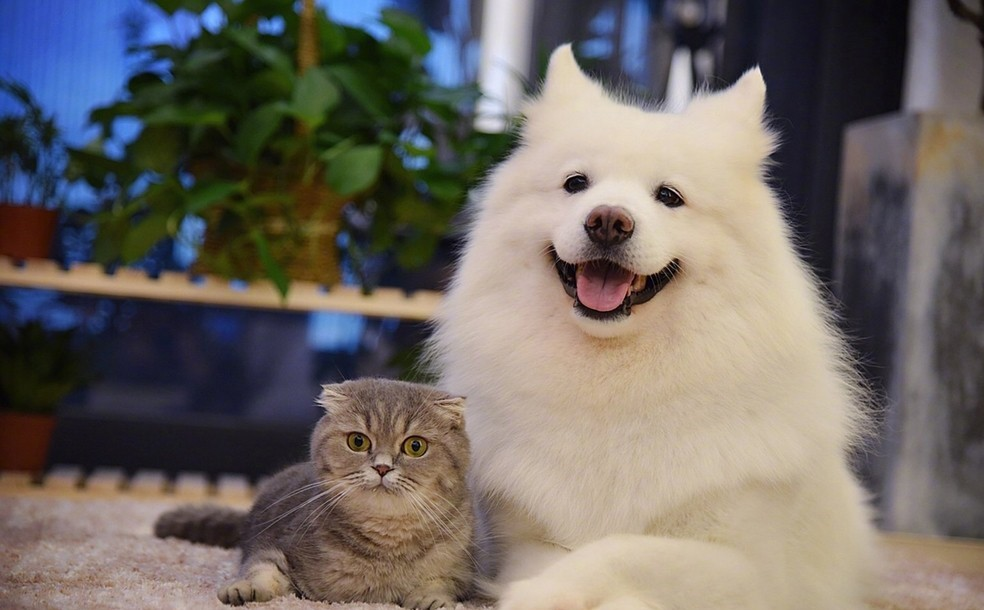
\includegraphics[width=0.4\textwidth]{1.jpg}
     \chartname{插入一副图}\label{fig:1}
\end{figure}

\begin{figure}
\begin{subfigure}{.48\textwidth}
  \centering
  \chartname{子图标题}\label{fig:2a}
  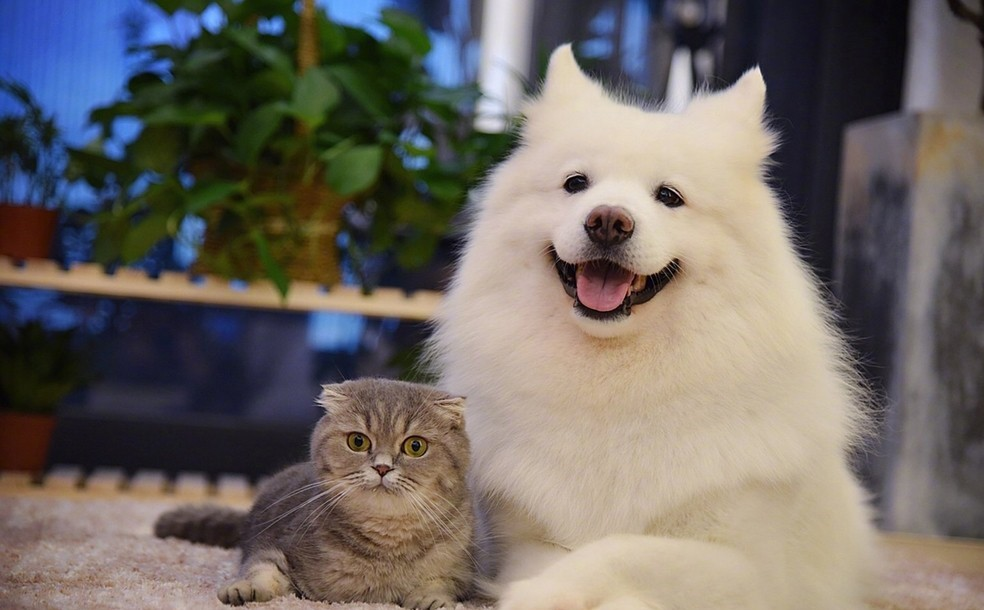
\includegraphics[width=.8\linewidth]{1.jpg}  
\end{subfigure}
\hfil
\begin{subfigure}{.48\textwidth}
  \centering
  \chartname{子图标题}\label{fig:2b}
  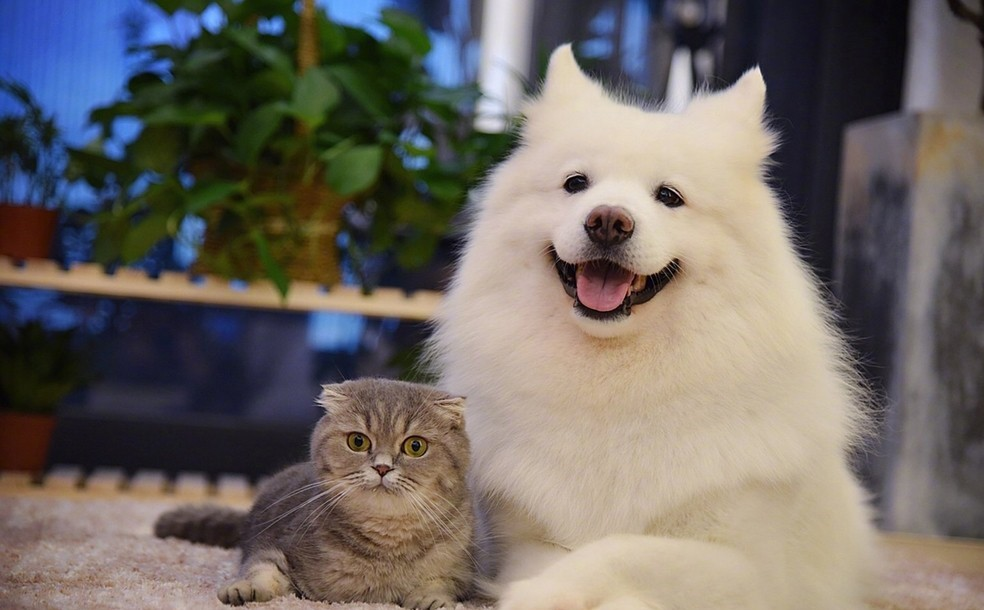
\includegraphics[width=.8\linewidth]{1.jpg}
\end{subfigure}
\chartname{两图并排,共享大标题,各有小标题}\label{fig:2}
\end{figure}

\begin{figure}[!htb]
\begin{subfigure}{.3\textwidth}
  \centering
  \chartname{子图标题}\label{fig:3a}
  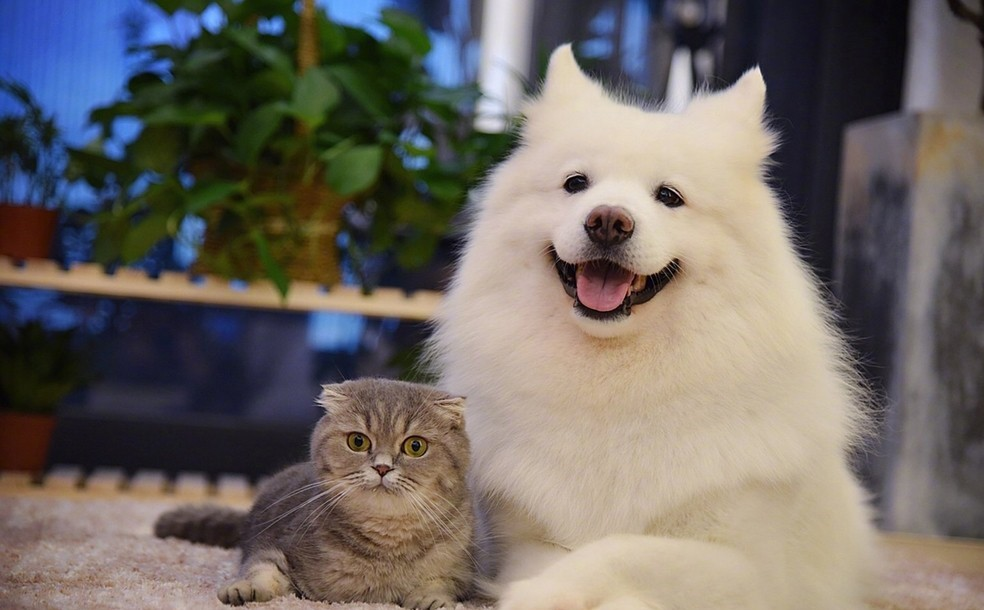
\includegraphics[width=.8\linewidth]{1.jpg}
\end{subfigure}
\hfil
\begin{subfigure}{.3\textwidth}
  \centering
  \chartname{子图标题}\label{fig:3b}
  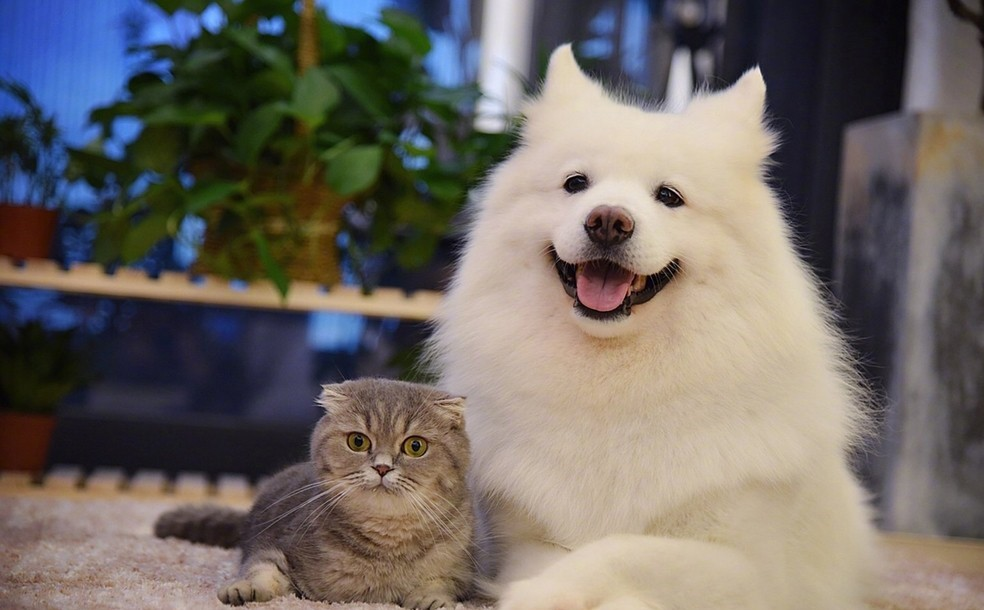
\includegraphics[width=.8\linewidth]{1.jpg}
\end{subfigure}
\hfil
\begin{subfigure}{.3\textwidth}
  \centering
  \chartname{子图标题}\label{fig:3c}
  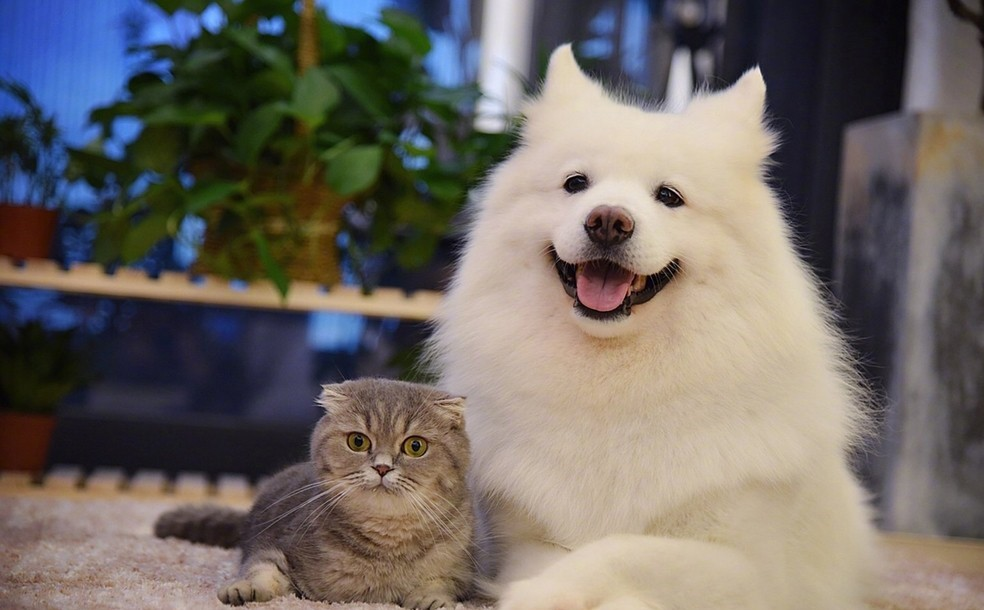
\includegraphics[width=.8\linewidth]{1.jpg}
\end{subfigure}
\vspace{3mm}
\newline   %此为换行命令,以此分割多子图两行
\begin{subfigure}{.3\textwidth}
  \centering
  \chartname{子图标题}\label{fig:3d}
  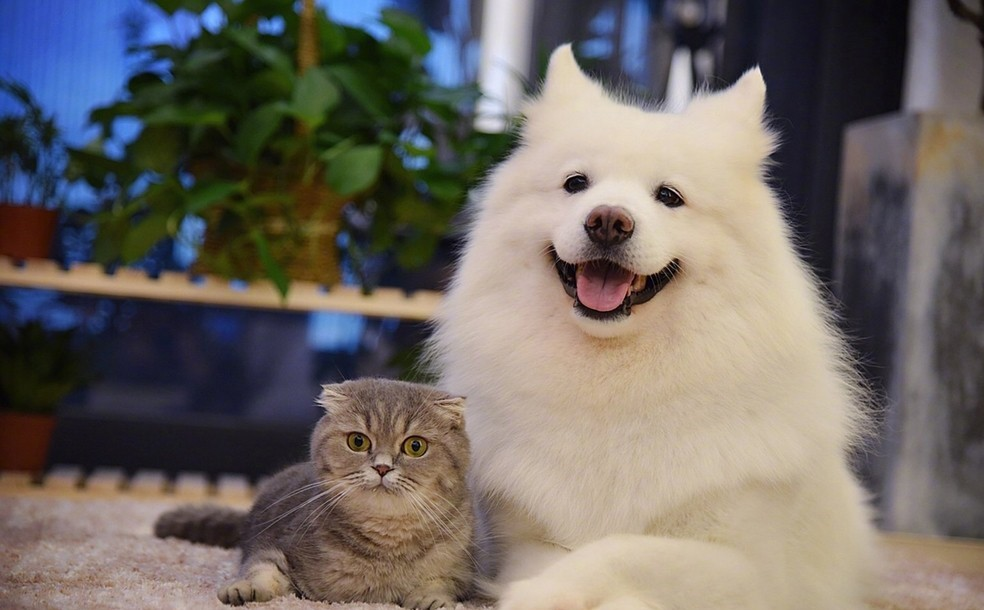
\includegraphics[width=.8\linewidth]{1.jpg}
\end{subfigure}
\hfil
\begin{subfigure}{.3\textwidth}
  \centering
  \chartname{子图标题}\label{fig:3e}
  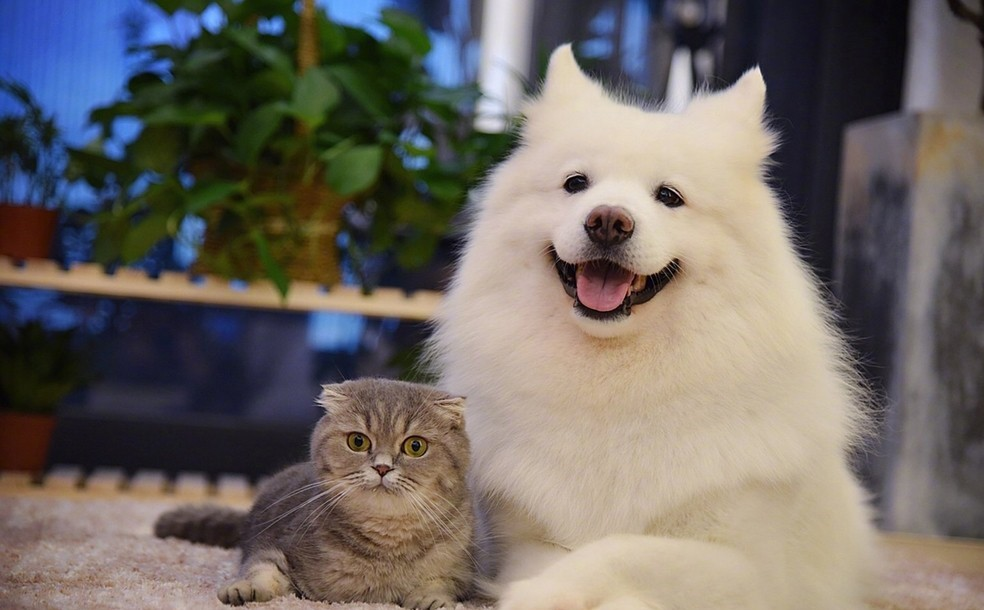
\includegraphics[width=.8\linewidth]{1.jpg}
\end{subfigure}
\hfil
\begin{subfigure}{.3\textwidth}
  \centering
  \chartname{子图标题}\label{fig:3f}
  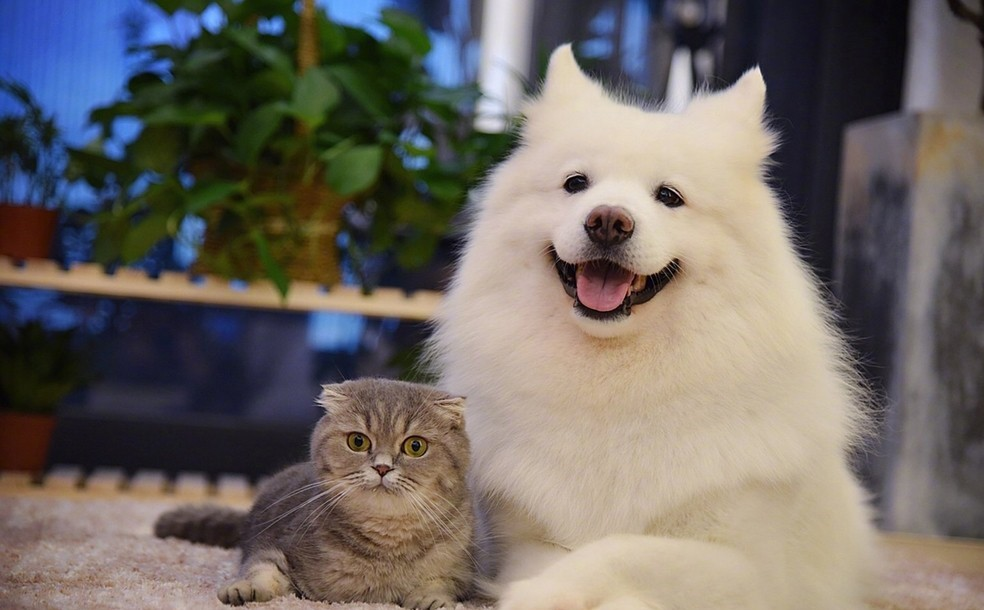
\includegraphics[width=.8\linewidth]{1.jpg}
\end{subfigure}
\vspace{3mm}
\newline   %此为换行命令,以此分割多子图两行
\begin{subfigure}{.3\textwidth}
  \centering
  \chartname{子图标题}\label{fig:3g}
  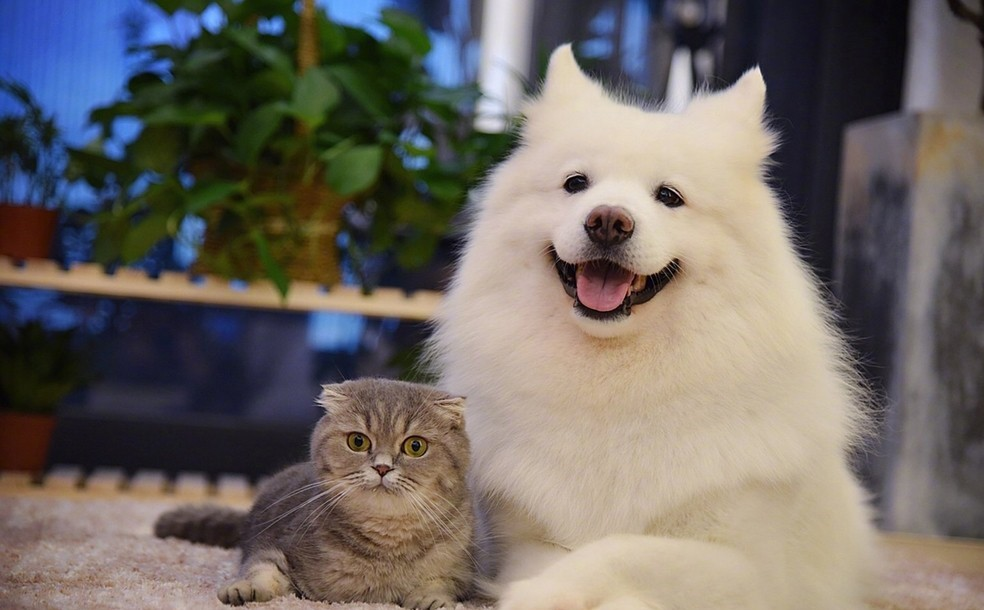
\includegraphics[width=.8\linewidth]{1.jpg}
\end{subfigure}
\hfil
\begin{subfigure}{.3\textwidth}
  \centering
  \chartname{子图标题}\label{fig:3h}
  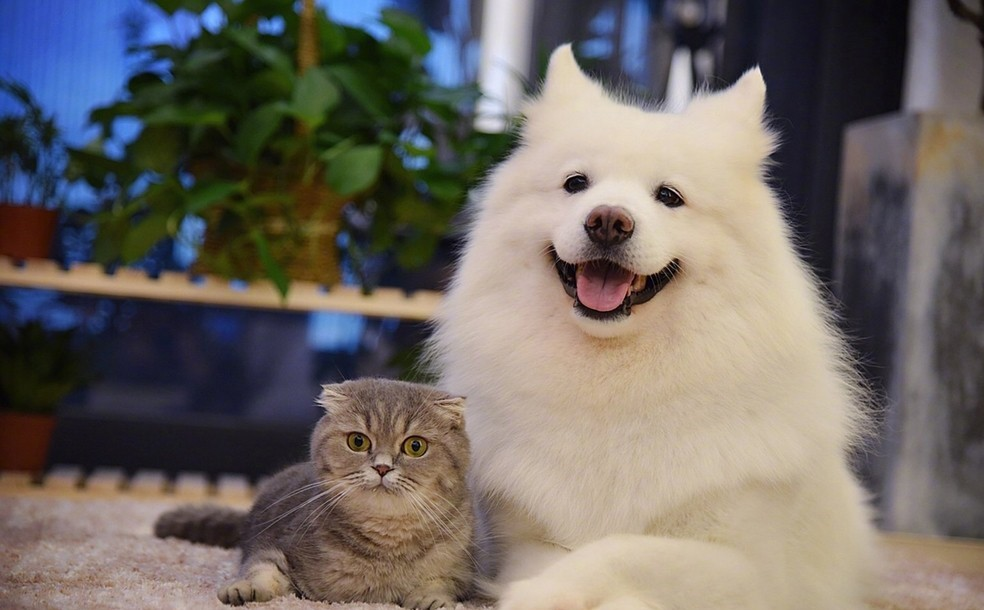
\includegraphics[width=.8\linewidth]{1.jpg}
\end{subfigure}
\hfil
\begin{subfigure}{.3\textwidth}
  \centering
  \chartname{子图标题}\label{fig:3i}
  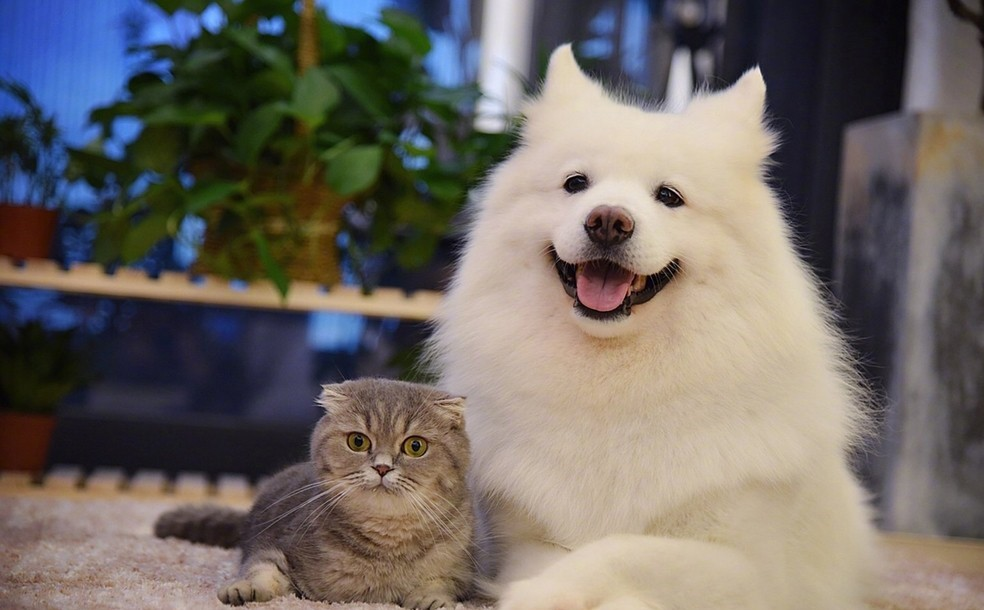
\includegraphics[width=.8\linewidth]{1.jpg}
\end{subfigure}
\chartname{多行多子图}\label{fig:3}
\end{figure}

\subsection{\LaTeX 常用的长度单位及度量}

考虑到插入图片需求的多样性,下面罗列了一些可以用于前面图片控制命令的\LaTeX 长度单位及命令,在具体使用的时候可以多尝试一下,以达到最佳效果。

需要特别说明的是\verb|\linewidth|和\verb|\textwidth|,前者指的是目前环境的宽度,是依赖于上下文的一个宽度值,例如新建了一个box,在这个box中,\verb|\linewidth|是box中文字的宽度。再例如minipage环境中,\verb|\linewidth|就和这个minipage的大小有关。而\verb|\textwidth|指的则是当前页面一行文字的宽度。

\begin{tabular}[!htb]{ll}
pt & 单位长度,大约为0.3515mm \\
mm & 一毫米 \\
cm & 一厘米 \\
in & 一英寸 \\
ex & 当前字体尺寸中x的高度 \\
em & 当前字体尺寸中M的宽度 \\
\verb|\columnsep| & 两列之间的距离 \\
\verb|\columnwidth| & 列宽 \\
\verb|\linewidth| & 当前环境的宽度 \\
\verb|\paperwidth| & 页面宽度 \\
\verb|\paperheight| & 页面高度 \\
\verb|\textwidth| & 文本宽度 \\
\verb|\textheight| & 文本高度 \\
\end{tabular}

\section{表格}

\subsection{通过在线工具生成表格}

表格的输入可能会比较麻烦,可以使用在线的工具,如~\unlink{https://www.tablesgenerator.com/}{Tables Generator}~能便捷的创建表格,也可以使用离线的工具,如~\unlink{https://ctan.org/pkg/excel2latex}{Excel2LaTeX}~支持从Excel表格转换成\LaTeX{}表格。\unlink{https://en.wikibooks.org/wiki/LaTeX/Tables}{LaTeX/Tables}~上及~\unlink{https://www.tug.org/pracjourn/2007-1/mori/mori.pdf}{Tables in LaTeX}~也有更多的示例能够参考。

\subsection{表格的一般形式}

表格环境一般格式如下:

\verb|\begin{table}[htbp]|\par 
\verb|\centering|\par 
\verb|\chartname{表名}|\par 
\verb|\label{表格标签}|\par 
\verb|\begin{tabular}{c c}|\par 
\verb|...&...\\|\par 
\verb|...&...|\par 
\verb|\end{tabular}|\par 
\verb|\end{table}|\par 

首先是关于插入表格的位置控制问题。

同前面的图片的插入一样,主要就是用$h,t,b,p$这四个选项来控制表格位于此处、页顶、页底及单独一页,笔者注意到从Tables Generator粘贴来的代码是没有给这一浮动体位置控制命令的,因此需要读者自己添加。

因为地物院的论文写作要求中图名位于下方,表名位于上方,所以在写表格的时候应当将生成表格标题以及表格标签的命令放在表格内容开始之前,也即是上面一般形式中的位置。

\subsection{分割单元格及单元格内容对齐}

表格的主体内容在\verb|\begin{tabular}{c l r}...\end{tabular}|之间,在两列之间插入\verb|&|字符作为分割,在两行之间插入\verb|\\|作为分割。
\par
在上面一般形式的\verb|\begin{tabular}{c c}|里第二个大括号中的$c$是控制表中两列单元格里的内容居中显示的意思,另外还有$l$和$r$,前者控制单元格内容左对齐,后者控制内容右对齐。

\subsection{使用在线工具的注意事项}

提醒一下使用在线工具的读者,就是表格标题的问题,Tables Generator这一工具,它不仅不给浮动体控制,也并不曾添加表名及表名标签命令。\par 因此请一定注意给自己复制过来的代码里加上生成表名及表名标签的命令,也就是\verb|\chartname{表名}\label{表格标签}|,这样在后续论文的写作中才能引用它。

\subsection{表格范例}

下面做一些表格的示例,读者可参照本模板源码以及所编译生成的表格来进行简单的表格编写。

\subsubsection{普通表格}

下面是一些普通表格的示例:

\begin{table}[htp]
  \centering
  \chartname{无框线表格}
  \label{tab:1}
  \begin{tabular}{ c c c }
 cell1 & cell2 & cell3 \\ 
 cell4 & cell5 & cell6 \\  
 cell7 & cell8 & cell9    
\end{tabular}
\end{table}

\begin{table}[htp]
  \centering
  \chartname{一般三线表}
  \label{tab:2}
  \begin{tabular}{ccc}
    \hline
    姓名& 学号& 性别\\
    \hline
    张三& 001& 男\\
    李四& 002& 女\\
    \hline
  \end{tabular}
\end{table}

\begin{table}[!htp]
  \centering
  \chartname{简单表格}
  \label{tab:3}
  \begin{tabular}{|l|c|r|}
    \hline
    姓名 & 单位 & 收入 \\
    \hline
    张三& 某腾 & 2W \\
    \hline
    李四& 某阿 & 1W \\
    \hline
    王五& 某团 & 3W \\
    \hline
  \end{tabular}
\end{table}

\begin{table}[!htp]
\centering
\chartname{组合行列表格}
\label{tab:4}
\begin{tabular}{ |c|c|c|c| } 
\hline
col1 & col2 & col3 \\
\hline
\multirow{3}{4em}{Multiple row} & cell2 & cell3 \\ 
& cell5 & cell6 \\ 
& cell8 & cell9 \\ 
\hline
\end{tabular}
\end{table}

\begin{table}[!htbp]
\centering
\chartname{定长表}
\label{tab:5}
\begin{tabular}{ |p{3cm}||p{3cm}|p{3cm}|p{3cm}| }
 \hline
 \multicolumn{4}{|c|}{Country List} \\
 \hline
Country Name or Area Name& ISO ALPHA 2 Code & ISO ALPHA 3 Code & ISO numeric Code \\
 \hline
 Afghanistan   & AF    &AFG&   004\\
 Aland Islands&   AX  & ALA   &248\\
 Albania &AL & ALB&  008\\
 Algeria    &DZ & DZA&  012\\
 American Samoa&   AS  & ASM&016\\
 Andorra& AD  & AND   &020\\
 Angola& AO  & AGO&024\\
 \hline
\end{tabular}
\end{table}

更多的表格样式可以看看Overleaf的帮助文档(点击菜单拉到底),Overleaf的帮助文档是比较全面的,基本上数学公式的排版、图片插入、图像绘制、表格创建等论文写作可能会用到的内容它都有讲解,读者可以多在这一文档里看看。

\subsubsection{统计表格}

创建占满整个文字宽度的表格需要使用到tabularx,如不需要,使用tabular就行。

\begin{table}[!htb]
  \centering
  \chartname{统计数据表格}
  \label{tab:6}
  \begin{tabularx}{\textwidth}{CCCC}
    \toprule
    姓名&年龄&身高&体重\\
    \midrule
    张三&14&156&42\\
    李四&16&158&45\\
    王二&14&162&48\\
    陈六&15&163&50\\
    \cmidrule{2-4} %添加2-4列的中线
    平均&15&159.75&46.25\\
    \bottomrule
  \end{tabularx}
\end{table}

\subsubsection{跨页表格}

跨页表格常用于附录(把正文放不下的实验数据统统放在附录的表中),以下是一个跨页表格的示例:

{\centering
  \begin{longtable}{ccccccccc}
  \chartname{跨页表格示例} \\
  \toprule
  组     & 甲 & 乙  & 丙  & 丁  & 戊  & 己  &  庚 & 辛 \\
  \midrule
  \endfirsthead

  \multicolumn{1}{l}{接上一页} \\
  \toprule
  组     & 甲 & 乙  & 丙  & 丁  & 戊  & 己  &  庚 & 辛 \\
  \midrule
  \endhead

  \bottomrule
  \hline \\
  \multicolumn{9}{r}{{转下一页}} \\
  \endfoot

  \bottomrule
  \endlastfoot    

  1     & 0 & 5  & 1  & 2  & 3  & 4  &  5 & 6 \\
  1     & 0 & 5  & 1  & 2  & 3  & 4  &  5 & 6 \\
  1     & 0 & 5  & 1  & 2  & 3  & 4  &  5 & 6 \\
  1     & 0 & 5  & 1  & 2  & 3  & 4  &  5 & 6 \\
  1     & 0 & 5  & 1  & 2  & 3  & 4  &  5 & 6 \\
  1     & 0 & 5  & 1  & 2  & 3  & 4  &  5 & 6 \\
  1     & 0 & 5  & 1  & 2  & 3  & 4  &  5 & 6 \\
  1     & 0 & 5  & 1  & 2  & 3  & 4  &  5 & 6 \\
  1     & 0 & 5  & 1  & 2  & 3  & 4  &  5 & 6 \\
  1     & 0 & 5  & 1  & 2  & 3  & 4  &  5 & 6 \\
  1     & 0 & 5  & 1  & 2  & 3  & 4  &  5 & 6 \\
  1     & 0 & 5  & 1  & 2  & 3  & 4  &  5 & 6 \\
  1     & 0 & 5  & 1  & 2  & 3  & 4  &  5 & 6 \\
  1     & 0 & 5  & 1  & 2  & 3  & 4  &  5 & 6 \\
  1     & 0 & 5  & 1  & 2  & 3  & 4  &  5 & 6 \\
  1     & 0 & 5  & 1  & 2  & 3  & 4  &  5 & 6 \\
  1     & 0 & 5  & 1  & 2  & 3  & 4  &  5 & 6 \\
  1     & 0 & 5  & 1  & 2  & 3  & 4  &  5 & 6 \\
  1     & 0 & 5  & 1  & 2  & 3  & 4  &  5 & 6 \\
  1     & 0 & 5  & 1  & 2  & 3  & 4  &  5 & 6 \\
  1     & 0 & 5  & 1  & 2  & 3  & 4  &  5 & 6 \\
  1     & 0 & 5  & 1  & 2  & 3  & 4  &  5 & 6 \\
  1     & 0 & 5  & 1  & 2  & 3  & 4  &  5 & 6 \\
  1     & 0 & 5  & 1  & 2  & 3  & 4  &  5 & 6 \\
  1     & 0 & 5  & 1  & 2  & 3  & 4  &  5 & 6 \\
  1     & 0 & 5  & 1  & 2  & 3  & 4  &  5 & 6 \\
  1     & 0 & 5  & 1  & 2  & 3  & 4  &  5 & 6 \\
  1     & 0 & 5  & 1  & 2  & 3  & 4  &  5 & 6 \\
  1     & 0 & 5  & 1  & 2  & 3  & 4  &  5 & 6 \\
  1     & 0 & 5  & 1  & 2  & 3  & 4  &  5 & 6 \\
  1     & 0 & 5  & 1  & 2  & 3  & 4  &  5 & 6 \\
  1     & 0 & 5  & 1  & 2  & 3  & 4  &  5 & 6 \\
  1     & 0 & 5  & 1  & 2  & 3  & 4  &  5 & 6 \\
  1     & 0 & 5  & 1  & 2  & 3  & 4  &  5 & 6 \\
  1     & 0 & 5  & 1  & 2  & 3  & 4  &  5 & 6 \\
  1     & 0 & 5  & 1  & 2  & 3  & 4  &  5 & 6 \\
  1     & 0 & 5  & 1  & 2  & 3  & 4  &  5 & 6 \\

  \end{longtable}
}

\section{列表}

\subsection{列表环境}

\begin{tabular}[htb]{l l}
\toprule
环境命令 & 命令含义\\
\midrule
\verb|\begin{enumerate}...\end{enumerate}| & 有序列表 \\
\verb|\begin{itemize}...\end{itemize}| & 无序列表 \\
\verb|\begin{description}...\end{description}| & 描述性列表 \\
\bottomrule
\end{tabular}\\

在一个列表环境中可以继续嵌套列表环境以实现更丰富的表现形式。

在列表环境中每个条目均以\verb|\item|命令开头,一个\verb|\item|即为一个条目。

当需要更改条目前的序号或符号时可以使用\verb|\item[...]|命令,在中括号中输入想要的序号或者符号即可。这一命令在描述性列表环境中,输入的应为描述性的文本内容。

\subsection{列表范例}

下面演示了创建有序列表、无序列表以及描述性列表,读者可参见本模板源码进行简单的列表编写。更多示例参见\unlink{https://www.latex-tutorial.com/tutorials/lists/}{LaTeX Lists}。

\subsubsection{有序列表}

有序列表即一个计数的使用序号来标识各条目的列表。
  \begin{enumerate}
      \item 第一条目
          \begin{enumerate}
              \item 第一条目中的第一项
              \item 第一条目中的第二项
          \end{enumerate}
      \item 第二条目
    \begin{enumerate}[label=(\roman*)]
      \item 第二条目中的第一项
      \item 第二条目中的第二项
    \end{enumerate}
      \item 第三条目
  \end{enumerate}

\subsubsection{无序列表}
  无序列表即一个不计数而使用符号来标识各条目的列表。
  \begin{itemize}
      \item 第一条目
      \begin{itemize}
          \item 第一条目中的第一项
          \item 第一条目中的第二项
      \end{itemize}
      \item 第二条目
      \item 第三条目
  \end{itemize}

\subsubsection{描述性列表}

描述性列表即一个用描述性文本来标识各条目的列表。

\begin{description}
  \item[Step 1]  条目一。
  \item[第二条]  条目二。
  \item[第三点]  条目三。
  \item[fourth]  条目四。
  \item[条目五]  条目五。
\end{description}

\section{参考文献}

\subsection{将文献添加到模板}

文献引用需要配合BibTeX使用,很多工具可以直接生成BibTeX文件(EndNote, NoteExpress, \unlink{https://xueshu.baidu.com/}{百度学术},\unlink{https://ac.scmor.com/}{谷歌学术})。\par 以百度学术为例,在其中找到一篇论文,点击\textbf{<引用>}按钮。在弹出来的窗口中点击导出至\textbf{<BibTeX>}按钮,将跳转页面的全部内容复制。 打开本模板ref.bib文件,将复制的内容空一行粘贴进去即可。

读者可以在每一篇文献的BibTeX内容代码的第一行大括号后进行命名,作用等同于引用其他内容所使用的标签。

\subsection{参考文献的罗列顺序}

本模板对参考文献的排序采用顺序编码制,也即文末参考文献的罗列顺序是与论文中的引用次序有关的,读者在论文中引用的第一篇文献会在参考文献页排在第一条,引用的第二篇文献则居于第二条,以此类推。

\section{论文中的引用}

\subsection{添加标签}

所谓标签也即是一种标识,为~\LaTeX~指明所需引用的对象。

故若要引用某一内容,需在该内容后添加标签,添加标签的命令为\verb|\label{...}|,大括号内为自行设定的标签文本。

添加标签时应注意标签的位置,例如一个编号的公式环境中只有一个公式时,标签命令置于公式内容之后或置于\verb|\begin{...}|之后,效用相同。但若是公式环境中有多个编号公式,则应将标签命令置于具体想要引用的那个公式之后。

对于图表的标签,一般均置于图名及表名命令之后。

\subsection{常用引用命令}

\begin{tabular}{l l}
  \verb|\ref{...}|   & 不带括号的引用 \\
  \verb|\eqref{...}|  & 引用公式所用的带括号引用 \\
  \verb|\pageref{...}| & 引用对象所在页码 \\
  \verb|\cite{...}| & 引用参考文献 
\end{tabular}

\subsection{插图的引用}

引用命令为\verb|\ref{...}|。

就像这样,如图\ref{fig:1},其描绘的是狸花猫与萨摩耶和谐相处的场景。\par 
如图\ref{fig:2a},其内容为猫狗照片。

\subsection{表格的引用}

引用命令为\verb|\ref{...}|。

就像这样:如表~\ref{tab:6}所示,统计表格一般是三线表形式。

\subsection{页码的引用}

引用命令为\verb|\pageref{...}|。

就像这样,就如上文第\pageref{fig:1}页的图\ref{fig:1}所示,图中为一猫一狗。

\subsection{文献的引用}

\begin{tabular}[htb]{l l l}
\toprule
命令 & 命令含义 & 效果\\
\midrule
\verb|\cite{...}| & 不带页码的引用 & \cite{r1} \\
\verb|\cite[...]{...}| & 带页码上标的引用 & \cite[255-261]{r1} \\
\verb|\pagescite{...}| & 自动页码的引用 & \pagescite{r1} \\
\verb|...\yearcite{...}| & 已有主语提供年份 & 杨文采\yearcite{r1} \\
\verb|\authornumcite[...]{...}| & 提供主语年份及页码的引用 & \authornumcite[255-261]{r1} \\
\bottomrule
\end{tabular}\\

另,引用多个文献时只需将各文献的标签以逗号分隔\verb|\cite{r1,r2,r3,r4,r5}|,效果如下:\cite{r1,r2,r3,r4,r5}。

特别说明,这里的文献引用,是从本模板的文献数据库,也即是$ref.bib$中引用,而非从网站或学术网站引用,读者需要将自己撰写论文所需的参考文献的BibTeX信息导入$ref.bib$文件中方可实现在论文中引用。